%%%%%%%%%%%%%%%%%%%%%%%%%%%%%%%%%%%%%%%%%
%
% CMPT 435
% Lab Zero
%
%%%%%%%%%%%%%%%%%%%%%%%%%%%%%%%%%%%%%%%%%

%%%%%%%%%%%%%%%%%%%%%%%%%%%%%%%%%%%%%%%%%
% Short Sectioned Assignment
% LaTeX Template
% Version 1.0 (5/5/12)
%
% This template has been downloaded from: http://www.LaTeXTemplates.com
% Original author: % Frits Wenneker (http://www.howtotex.com)
% License: CC BY-NC-SA 3.0 (http://creativecommons.org/licenses/by-nc-sa/3.0/)
% Modified by Alan G. Labouseur  - alan@labouseur.com
%
%%%%%%%%%%%%%%%%%%%%%%%%%%%%%%%%%%%%%%%%%

%----------------------------------------------------------------------------------------
%	PACKAGES AND OTHER DOCUMENT CONFIGURATIONS
%----------------------------------------------------------------------------------------

\documentclass[letterpaper, 10pt]{article} 

\usepackage[english]{babel} % English language/hyphenation
\usepackage{graphicx}
\usepackage{xcolor}
\graphicspath{ {./images/} }
\usepackage[lined,linesnumbered,commentsnumbered]{algorithm2e}
\usepackage{listings}

% Lstlistings configuration
\definecolor{codegreen}{rgb}{0,0.6,0}
\definecolor{codegray}{rgb}{0.5,0.5,0.5}
\definecolor{codepurple}{rgb}{0.58,0,0.82}
\definecolor{backcolour}{rgb}{0.95,0.95,0.92}

\lstdefinestyle{mystyle}{
    backgroundcolor=\color{backcolour},   
    commentstyle=\color{codegreen},
    keywordstyle=\color{magenta},
    numberstyle=\tiny\color{codegray},
    stringstyle=\color{codepurple},
    basicstyle=\ttfamily\footnotesize,
    breakatwhitespace=false,         
    breaklines=true,                 
    captionpos=b,                    
    keepspaces=true,                 
    numbers=left,                    
    numbersep=5pt,                  
    showspaces=false,                
    showstringspaces=false,
    showtabs=false,                  
    tabsize=2
}

\lstset{style=mystyle}
\lstset{language=Java}

\usepackage{fancyhdr} % Custom headers and footers
\pagestyle{fancyplain} % Makes all pages in the document conform to the custom headers and footers
\usepackage{lastpage}
\usepackage{wasysym}
\usepackage{url}

% Set up for minted package. It had some bugs so I decided to only keep lstlistings.
% \usepackage{minted}
% \makeatletter
% \newlength\minted@belowskip
% \define@key{minted@opt}{belowskip}[\@topsepadd]
% {\setlength{\minted@belowskip}{#1}}

% \def\minted@endparenv{%
%   \addpenalty\@endparpenalty\addvspace\minted@belowskip\@endpetrue}
% \def\FV@EndList{%
%   \FV@ListProcessLastLine
%   \FV@EndListFrame
%   \minted@endparenv
%   \endgroup
%   \@endpetrue}
% \makeatother
% \newminted{java}{linenos=true, belowskip=3cm}

\fancyhead{} % No page header - if you want one, create it in the same way as the footers below
\fancyfoot[L]{} % Empty left footer
\fancyfoot[C]{page \thepage\ of \pageref{LastPage}} % Page numbering for center footer
\fancyfoot[R]{}

\renewcommand{\headrulewidth}{0pt} % Remove header underlines
\renewcommand{\footrulewidth}{0pt} % Remove footer underlines
\setlength{\headheight}{13.6pt} % Customize the height of the header

%----------------------------------------------------------------------------------------
%	TITLE SECTION
%----------------------------------------------------------------------------------------

\newcommand{\horrule}[1]{\rule{\linewidth}{#1}} % Create horizontal rule command with 1 argument of height

\title{	
   \normalfont \normalsize 
   \textsc{CMPT 435 - Fall 2021 - Dr. Labouseur} \\[10pt] % Header stuff.
   \horrule{0.5pt} \\[0.25cm] 	% Top horizontal rule
   \huge Assignment Three - Searching and Hashing \\     	    % Assignment title
   \horrule{0.5pt} \\[0.25cm] 	% Bottom horizontal rule
}

\author{Augusto Gonzalez-Bonorino \\ \normalsize augusto.gonzalezbonorino1@marist.edu}

\date{\normalsize\today} 	% Today's date.

\begin{document}

\maketitle % Print the title

%----------------------------------------------------------------------------------------
%   CONTENT SECTION
%----------------------------------------------------------------------------------------

% - -- -  - -- -  - -- -  -

\section{Description of the program}

The program described in the following sections has the goal of implementing and analyzing searching algorithms (Linear and Binary search specifically) and hashing to optimize retrieval of information. This documentation is organized in the following way: 1) Description of the program; 2) Explanation of the problem tackled by searching algorithms; 3) Description of my Linear search implementation' details; 4) Description of my Binary search implementation's details; 5) Conceptual description of hashing and the details of my java code as well as the method employed to handle collisions; 6) Explanation of the main elements of Main class; 7) Results and Further thoughts.
\\
\\
\begin{center}
    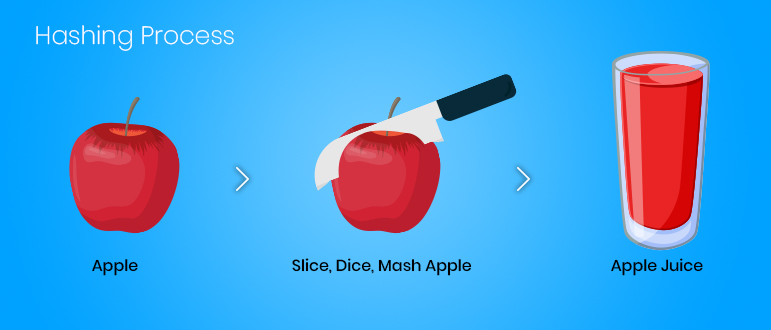
\includegraphics[scale=0.40]{images/Hashing-definition.jpg}
\end{center}
\\
\section{Searching}
\\
\\
Searching addresses, as you may have inferred from its name, the issue of searching (and finding) a particular element among many other elements. It seems simple at first, you may be wondering why not just go checking one by one until you find it? Well, fair enough, that is a potential approach; it is called Linear Search and we will dive deeper into its implementation in Java soon. But, what if you have 9 billion elements to search? Well, assuming you get very lucky you might find it very quickly if it is at the beginning of the list or very unlucky if it is at the end. It is just too much data to go checking each one of them, Linear search worst case is O(n) when the element is at the end or $\Omega (\frac{n}{2})$ on average. But we can surely do better, right? This is exactly the question that computer scientists are interested in answering when designing searching algorithms. An alternative, which we will examine as well, is Binary Search. If you recall the idea behind Merge sort then you may find the inner workings of Binary search extremely familiar. Basically, given a \textbf{sorted} array, we split it in half, check if the element (i.e. key or target) being searched is equal, greater than or smaller than the element that was chosen to split the list at. Then, continue to do that until the element is found or the whole list is traversed (meaning that the element was not found). If this sounds a little bit confusing consider the following illustration of Binary Search:
\\
\begin{center}
    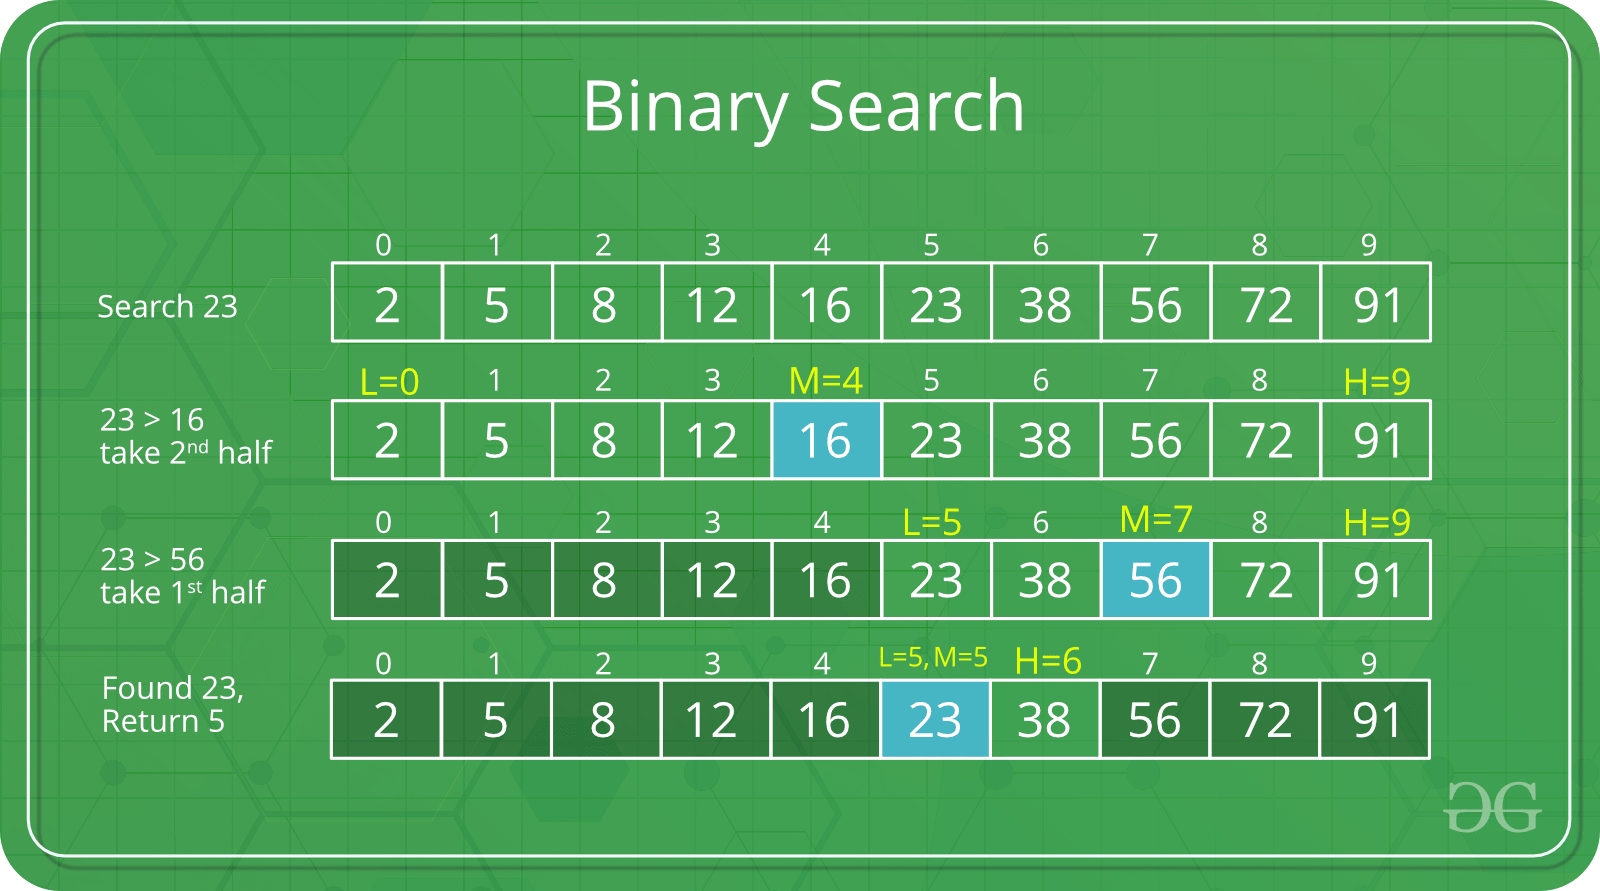
\includegraphics[scale=0.20]{images/Binary-Search.png}
\end{center}
\\
Due to its "halving" approach the algorithm is able to improve its performance significantly compared to Linear search with its worst case being $O(log\hspace{0.5mm} n)$. For completion purposes, I believe it is important to emphasized the requirement of having a sorted array when implementing Binary Search. The sorting algorithm's complexity must also be taken into account when calculating the performance of the program. I chose to use Quick sort in this project since it is the best performing algorithm we have seen in the class so far, and so the total complexity for Binary search's worst case would be $O(log n) + O(n^2)$. 
\\
\\
\section{Linear Search}
\\
\\
Our first attempt to solve the aforementioned problem comes in the name of Linear Search. You will most likely find this algorithm  intuitive and easy to understand. Here is my implementation in Java:
\begin{lstlisting}
public static int linearSearch(String[] arr, String key){ 
	
	int idx = 0;
	
	for(int i=0;i<arr.length;i++)
	{
		
		linearSearchComparisons++;
        if(arr[i].compareToIgnoreCase(key) == 0)
        {    
        	
            return i;    
            
        } // if  
        
    } // for loop
	
    return linearSearchComparisons;
    
} // linearSearch
\end{lstlisting}
It is also known as "brute" search because, given an array of length \textit{n}, it checks element by element to see if any of them matches the key (i.e. target). Thus, the worst case is $O(n)$ if the key is all the way at the end of the list, the average case is $\Omega (\frac{n}{2})$. You might think, well but computers are fast so it shouldn't be a problem. Well, it is not for the most part but imagine having to look for one element in a list of 50 billion elements. Yes, we would get it done but we surely can be smarter about it. Enter Binary Search.
\\
\\
\section{Binary Search}
\\
\\
Given a \textbf{sorted} array - and it has to be sorted - of length \textit{n}, Binary Search algorithm iteratively splits the array (and sub-arrays) in half until the target is found or the whole list is traversed. Since after every split you are effectively eliminating one half of the array we compute the asymptotic performance to be $O(\log n)$. Here is my implementation in Java:
\begin{lstlisting}
public static int binarySearch(String[] arr, String key)
{
    int start = 0;
    int mid = 0;
    int stop = arr.length - 1;
    int pos = 0;
    int idx = -1;;
    int comps = 0;
    
    while (start <= stop && idx == -1)
    {
    	binarySearchComparisons++;
    	
    	comps++;
    	
    	mid = start + (stop - start) / 2;
    	
    	pos = key.compareToIgnoreCase(arr[mid]);
    	
    	// if items are equal update the index
    	if (pos == 0)
    		idx = mid;
    	
    	// if key is greater update starting point
    	if (pos > 0)
    		start = mid + 1;
    	
    	// if key is smaller update end point
    	else
    		
    		stop = mid - 1;
    	
    } // while
	
	
    return comps;
    
} // binarySearch
\end{lstlisting}
The function takes in an array of Strings and a key value to look for. Remember I mentioned we split the array in half? Well, line 16 defines the middle of an array. We will use the default value of starting point 0 and ending point 1 less than the length of the array, but note that if the starting point were to be greater than 0 then the midpoint would be different and so I accounted for that with $"(stop - start)"$. Then, we compare the value of the midpoint with the key and decide if we should split and go left or right. If it is greater we will go right and keep searching \textit{while} the element is not found and the starting point is not greater than the stop point. My implementation returns the number of comparisons since it was part of the assignment but it can easily be updated such that it returns the index instead. We improved a lot with Binary search, but can we do even better? Enter Hashing.

\pagebreak
\section{Hash Table with chaining}
\\
\\
A Hash table is a data structure that maps keys to values (just like a dictionary) by indexing each element inserted into it to optimize retrieval performance. The main idea behind hashing is to distribute key/value pairs across an array of pointers or "buckets" in the hash table. The hash table is often implemented as an array of Linked lists containing the indexed elements. This index is generated by what's called a "hash function". Therefore, if you want to insert an element to the hash table your algorithm should first generate an index (i.e. hash code) to determine where to place that element. Why do you need a function to create an index? You might be asking. Well, this is a very special type of index because is custom made. By custom made I mean the following: a certain property of the elements is chosen (the length of the String in this case) and some operations are performed to transform such property into a unique number linked to the element inserted (in our case convert characters to ASCII and sum each value). At this point, you might find it beneficial to look at how all of this is actually implemented. Here is my implementation:
\begin{lstlisting}
/**
	 * local class definition for our custom object used to store the key/value pair in the hash table
	 * @author Bonoc
	 *
	 */
    public static class HashObject {
        public String key;
        public String value;
    }
\end{lstlisting}
First, I decided to define my own object to store the key/value pairs. I called it \textbf{HashObject}. Next, we intialize the size of the hash table and our array of linked lists:
\begin{lstlisting}
/**
     * Constant to hold the maximum size of the hash table
     */
    public static final int HASH_TABLE_SIZE = 250;

    /**
     * Linked list of custom HashObject class which simply stores a key and a value.
     */
    @SuppressWarnings("unchecked")
	private LinkedList<HashObject>[] arr = new LinkedList[HASH_TABLE_SIZE];

    /**
     * Constructor
     */
    public HashTableGonzalezBonorino() {
    	
        //init vals in array
        for(int i=0; i<HASH_TABLE_SIZE; i++) {
            arr[i] = null;
            
        } // for loop
        
    } // HashTableGonzalezBonorino
\end{lstlisting}
Pretty straightforward. Now, we need to be able to populate our hash table. For this, I have defined the following function to insert (or \textbf{put}) elements into it:
\begin{lstlisting}
/** 
     * Method to insert an element into the hash table
     * @param key
     * @param value
     */
    public void put(String key, String value) {
    	int index = makeHashCode(key);
        LinkedList<HashObject> items = arr[index];

        if(items == null) {
            items = new LinkedList<HashObject>();

            HashObject item = new HashObject();
            item.key = key;
            item.value = value;

            items.add(item);

            arr[index] = items;
        } // if
        
        else 
        {
            for(HashObject item : items) 
            {
                if(item.key.equals(key)) 
                {
                    item.value = value;
                    return;
                } // if
                
            } // for each

            HashObject item = new HashObject();
            item.key = key;
            item.value = value;

            items.add(item);
            
        } // else
        
    } // put
\end{lstlisting}
The function takes in the String key/value pair, creates a hash code (index) for it and adds it to the list of linked lists at that index. Next, if the space is null then create a new linked list, add it to the array and populate a \textbf{HashObject} with the two Strings. Else, if there is already a linked list at that index then "chain" both objects by creating a pointer to the new element. The use of linked lists simulates a line of nodes "chained" to each other and thus the name "chaining" to avoid that the two objects collide. 
\\
For this particular assignment we have no use for a delete method, but I decided to include one for completion purposes. I won't go into much detail about it but here is my \textit{delete} function:
\begin{lstlisting}
/**
     * Method to delete item from hash table
     * @param key
     */
    public void delete(String key) {
        int index = makeHashCode(key);
        LinkedList<HashObject> items = arr[index];

        if(items == null)
            return;

        for(HashObject item : items) 
        {
            if (item.key.equals(key)) 
            {
                items.remove(item);
                return;
                
            } // if 
            
        } // for each
        
    } // delete
\end{lstlisting}
\\
Very well. I mentioned hash code and hash function many times already in previous paragraphs. Recall that the method I employed was converting each character to ASCII and summing all those numbers. Here is how that looks like in Java:
\begin{lstlisting}
/**
     * Method to generate hash code for indexing
     * @param key
     * @return hash code generated
     */
    public static int makeHashCode(String key) {
   	 
    	key = key.toUpperCase();
        int length = key.length();
        int letterTotal = 0;

        // Iterate over all letters in the string, totalling their ASCII values.
        
        for (int i = 0; i < length; i++) 
        {	
           char thisLetter = key.charAt(i);
           int thisValue = (int)thisLetter;
           letterTotal = letterTotal + thisValue;
           
        } // for loop

        // Scale letterTotal to fit in HASH_TABLE_SIZE.
        int hashCode = (letterTotal * 1) % HASH_TABLE_SIZE;  // % is the "mod" operator
        
        // TODO: Experiment with letterTotal * 2, 3, 5, 50, etc.
        // ANS: It takes a greater number of comparisons to find an element

        return hashCode;
        
     	} // makeHashCode
\end{lstlisting}
First, we make every character upper case to normalize the values. Then, we convert each character of the given String to an integer (ASCII value) and sum over all those values to obtain \textit{letterTotal}. Lastly, we take that number and divide it by the size of the hash table to get our acclaimed hash code.
\\
There is one last component of our Hash Table, which is getting an object (i.e. retrieving it). Well, we need an index to find the element and then loop through every element located at that index (if there is only one element then it just one loop). We know how to get the index, use the hash function we just went over, and checking is straightforward. Here is my implementation in Java:
\begin{lstlisting}
/**\
     * Method to get object (HashObject) from the hash table
     * @param key
     * @return item if found null if not found
     */
    private HashObject getObj(String key) {
    	
    	
        if(key == null)
            return null;

        int index = makeHashCode(key);
        LinkedList<HashObject> items = arr[index];
        
        if(items == null)
            return null;
        
		// for each item in items
        for(HashObject item : items) {
        	
        	// if we find it end the loop and return item
            if(item.key.equals(key))
            {
                return item;
            } // if
            
        } // for each
        
    return null;    
    } // getObj
\end{lstlisting}
Note, first we make sure that the key given as input is not null. Next, we create our index using our hash function \textit{makeHashCode} and initialize an array of linked lists. It follows that, if the list \textit{items} is not empty, we check if any of the elements in that bucket is equals to our \textit{key} element. If we find it, return the value otherwise return null. But, there is a little detail I needed to address. We are asked to count and print out the comparisons of each query. Yet, my \textit{getObj} function only returns the value. To solve this I added an additional method, which I named \textit{getObjComps} that performs the exact same routine as \textit{getObj} but returns the comparisons (or an arbitrary integer if element is not found) made to find the element instead of the value. Here is how I modified the above-mentioned function to get the comparisons:
\begin{lstlisting}
/**
     * Method to get the total number of comparisons made per query
     * @param key
     * @return number of comparisons
     */
	public int getObjComps(String key) {
		
		int hashTableComparisons = 0;
		
	    if(key == null)
	        return -5;
	
	    int index = makeHashCode(key);
	    LinkedList<HashObject> items = arr[index];
	    
	    
	    if(items == null)
	        return -5;
	    
		
	    for(HashObject item : items) {
	    	
	    	hashTableComparisons++;
	    	
	        if(item.key.equals(key))
	        {
	                return hashTableComparisons;
	            } // if
	        } // for each
	    
	    return -5;
	} //getObjComps
\end{lstlisting}
\pagebreak
\section{Main}
\\
\\
Before concluding this documentation with the results obtained I wanted to briefly explain the mechanics of the Main class. The first half of the code simply contains the initialization of our variables and objects to be utilized and reads every element from our beloved "magicitems.txt" file. 
\begin{lstlisting}
/**
 * 
 * @author Augusto Gonzalez Bonorino <br>
 * 
 * assignment1GonzalezBonorino <br>
 * Due Date and Time: 09/24/21 <br><br>
 *
 * Purpose: Develop program that leverages a singly linked list, stacks and queues to find palindromes. <br><br>
 *			
 * Input: A text file containing the words or sentences to check for palindromes.
 * 		  
 * Output: The program prints out those words or sentences that were indeed palindromes.<br><br>
 *		   
 *
 * Certification of Authenticity: <br>
 * 
 * I certify that this assignment is entirely my own work. <br>
 */
public class MainGonzalezBonorino {
	
	static Scanner keyboard = new Scanner(System.in);
	
	private static final String FILE_NAME = "magicitems.txt";
	private static final int FILE_LEN = 666;
	
	static int linearSearchComparisons = 0;
	static int binarySearchComparisons = 0;
    static int avgHashComps = 0;

	
	public static void main(String[] args) {
		
		File theMagicFile = null;
		QuickSortGonzalezBonorino sort = new QuickSortGonzalezBonorino();
		
		String tempString = null;

		String [] myMagicList = new String[FILE_LEN];
		
		int numItems = 0;
		
		String ans = "\nSome suggestions: \n"
				+ "\n* Check that the name of the file was typed correctly"
				+ "\n* Make sure that you are not missing any information in your item description in the file"
				+ "\n* Make sure you are not entering more or less items than specified";
		
		try
		{
			
			theMagicFile = new File(FILE_NAME);
			
			Scanner input = new Scanner(theMagicFile);
			
			while(input.hasNextLine()) {
				
				tempString = input.nextLine();
				myMagicList[numItems] = tempString;
				
				numItems++;
				
			} //while 
			
			input.close();
			
		} //try
		
		catch(IndexOutOfBoundsException ex)
	    {
			System.out.println("Oops, something went wrong!");
			System.out.println("It seems that the program has reached an index out of bounds.");
			
	    } // catch index out of bound
\end{lstlisting}
I accounted for multiple more exceptions but I have decided to omit them in the document for conciseness. Now, the second half is where the magic happens. Recall that every algorithm takes in a \underline{sorted array}, thus it seems reasonable to sort our array before anything else. I achieve this by re-utilizing the \textit{\textbf{Quick Sort}} algorithm we developed for our previous assignment. Next, I instantiate a \textit{Random} object which I use to generate the 42 random integers we will use to index the full \textit{myMagicList} array. To do so, we first create a regular array to store our 42 randomly picked elements. Then, we populate it by using our random integer generator to create random indexes used to retrieve elements from the original list. Here is how that code looks like:
\begin{lstlisting}
		// Quick Sort
		
		System.out.println(sort.quickSort(myMagicList, 0, myMagicList.length - 1));
		
		// Select 42 random items for sorted myMagicList
		// Add random items to temporary array of strings
		
		Random rand = new Random();
		String [] tempMagicList = new String[42];
		
		// loop to generate 42 random numbers to randomly index myMagicList
		
		for (int i = 0; i < tempMagicList.length; i++)
		{ 
			
			int idx = rand.nextInt(FILE_LEN);
			
			tempString = myMagicList[idx];
			
			tempMagicList[i] = tempString;
			
			
		} // for loop
		
		// double check that elements in tempMagicList are random
		
		for (int j = 0; j < tempMagicList.length; j++)
		{
			System.out.println(tempMagicList[j]);
			
		} // for loop
\end{lstlisting}
Lastly, the last third of the class simply implements the three searching (or retrieving) algorithms previously discussed and prints out the total number of comparisons as well as the average number of comparisons it took each of them to find the 42 randomly picked elements from \textit{tempMagicList} in the original \textit{myMagicList}. The code is straightforward, thus I will abstain from providing detailed explanation of its design. Here is the Java code:
\begin{lstlisting}
        // Linear Search
		
		//LinearSearchGonzalezBonorino linearSearch = new LinearSearchGonzalezBonorino();
		
		// use linear search to look for each of the 42 random items and print comparisons
		

		int avgComparisonsLS = 0;
		
		System.out.println("LINEAR SEARCH");
		System.out.println("*********************************************");
		System.out.println(" ");
		
		for (int k = 0; k < tempMagicList.length; k++)
		{
			
			System.out.println("Comparisons made with linear search to find element "+ tempMagicList[k] + ": " + linearSearch(myMagicList, tempMagicList[k]));
			
			avgComparisonsLS += linearSearch(myMagicList, tempMagicList[k]);
			
			
		} // for loop
		
		// Compute and print average number of comparisons for LS
		
		avgComparisonsLS /= tempMagicList.length;
		
		System.out.println(" ");
		
		System.out.println("Average Comparisons for Linear Search: " + avgComparisonsLS);
		
		System.out.println(" ");
		
		
		
		// Binary Search
		
		//BinarySearchGonzalezBonorino binarySearch = new BinarySearchGonzalezBonorino();
		
		// use binary search to look for each of the 42 random items and print comparisons
		
		int avgComparisonsBS = 0;
		
		System.out.println("BINARY SEARCH");
		System.out.println("****************************************************");
		System.out.println(" ");
		
		for (int k = 0; k < tempMagicList.length; k++)
		{
			
			System.out.println("Comparisons made with binary search to find element "+ tempMagicList[k] + ": " + binarySearch(myMagicList, tempMagicList[k]));
			
			avgComparisonsBS += binarySearch(myMagicList, tempMagicList[k]);
			
			
		} // for loop
		
		// Compute and print average number of comparisons for BS
		
		avgComparisonsBS /= tempMagicList.length;
	
		System.out.println(" ");
		
		System.out.println("Average Comparisons for Binary Search: " + avgComparisonsBS);
		
		System.out.println(" ");
		

		// Hashing
		
        System.out.println("HASH TABLE");
        System.out.println("*************************************************");
        System.out.println(" ");
		
        // Instantiate HashTableGonzalezBonorino object
        
        HashTableGonzalezBonorino hash = new HashTableGonzalezBonorino();
       
        // Populate it with all the elements in magic list 
        
        for (int h = 0; h < myMagicList.length; h++)
        {
        	
        	hash.put(myMagicList[h], myMagicList[h]);
        	
        } // for loop
        
        // Search for each of the 42 randomly selected items and print the total number of comparisons
        for (int a = 0; a < tempMagicList.length; a++)
        {
        	int localComps = 0;
        	int globalComps = 0;
        	
        	System.out.println("Looking for: " + hash.get(tempMagicList[a]));
        	System.out.println("Hash comparisons: " + hash.getObjComps(tempMagicList[a]));
        	
        	globalComps = hash.getObjComps(tempMagicList[a]);
        	
        	localComps = globalComps + 1; 
        	
        	avgHashComps += localComps;
        	System.out.println("total comps: " + avgHashComps);
        	System.out.println();
        	
        } // for loop
        
        System.out.println("Overall Average Comparisons for Hash Table: " + avgHashComps / tempMagicList.length);

	} // main
\end{lstlisting}
The key detail to note is that just by trading a little bit of extra space the Hash Table lets us perform lighting fast operations in constant time to retrieve the elements we are looking for. Great! Now that we are familiar with the entire program let's take a look at some performance metrics.
\pagebreak
\section{Results and Further thoughts}
\\
\\
Recall the Asymptotic analysis for each algorithm:
\begin{itemize}

    \item Linear Search $\rightarrow O(n)$ and $\Omega (\frac{n}{2})$
    
    \item Binary Search $\rightarrow O(log\hspace{0.5mm} n)$ and $\Omega (log\hspace{0.5mm} n)$
    
    \item Hash Table $\rightarrow O(1 + \alpha)$ and $\Omega (1 + \alpha)$
\end{itemize}
please have these characteristics in mind while looking at the metrics and remember that the length of the file we are traversing is 666 and the complexity of Quick Sort is $O(n^2)$.
\begin{table}[hdt]
    \centering
    \begin{tabular}{|l|l|}
        \hline
        Algorithm     & Average Comparisons \\ \hline
        Linear Search & 284                 \\ \hline
        Binary Search & 9                   \\ \hline
        Hash Table    & 3                   \\ \hline
    \end{tabular}
\end{table}
\\
Those numbers look a lot like what our analysis predicted. Linear search oscillates around the range 280-360 comparisons which on average gives 333 (half the length of our list). Binary search makes 9 comparisons on average and Hash table makes only 3 on average! That's a great improvement if you ask me for giving up only a little extra space.
\\
In the future, we could update this program to count not only the comparisons but the time and space each of them took in order to obtain a much better analysis of each algorithms complexity. I have a confession. I tried implementing Binary Search recursively and counting its comparisons gave me such a headache that the least I can do is joke about it. For that, here is a joke a famous astrophysicist, Niel DeGrasse Tyson, tweeted last year:
\\
\begin{center}
    
\includegraphics[scale=0.35]{images/recursions_joke.jpg}
\end{center}
\end{document}
